% Diagrama de bloques de hardware del nodo ESP32 (reglas B1-B6, anti-generico).
% Fuente de verdad: docs/hardware-spec.md. Elementos [CONFIRMAR] en trazo discontinuo
% (P-06: ubicacion del shunt; P-07: VCC/pull-up DHT11 y ciclo del calentador MQ-7).
% Ancho natural <= 13.6 cm (1 columna acmsmall), sin escalar: fuente minima 7 pt.
\documentclass[tikz,border=4pt]{standalone}
\usepackage[utf8]{inputenc}
\usepackage[T1]{fontenc}
\usepackage{lmodern}
\usetikzlibrary{shapes.geometric, arrows.meta, positioning, fit, backgrounds, calc}

\definecolor{acento}{RGB}{176,30,30}   % unico color de acento: energia

\tikzset{
  base/.style      = {draw, thick, align=center, font=\fontsize{7.5}{8.3}\selectfont,
                      inner sep=1.5pt, minimum height=7.5mm},
  sensor/.style    = {base, fill=gray!12, minimum width=19mm, text width=18mm},
  actuator/.style  = {base, fill=gray!12, minimum width=19mm, text width=18.5mm},
  mcu/.style       = {base, very thick, fill=gray!28, minimum width=26mm, minimum height=34mm},
  iface/.style     = {base, fill=white, minimum width=8.5mm, minimum height=6mm,
                      font=\fontsize{7}{7.6}\selectfont, inner sep=1pt},
  power/.style     = {base, draw=acento, very thick, fill=white, minimum width=22mm},
  confirmar/.style = {dashed},
  data/.style      = {-{Stealth[length=2mm]}, thin, black},
  pwr/.style       = {-{Stealth[length=2.3mm]}, line width=1.3pt, acento},
  lbl/.style       = {font=\fontsize{7}{7.5}\selectfont, inner sep=1pt},
  tag/.style       = {font=\fontsize{7}{7.5}\selectfont\bfseries, text=acento, inner sep=1pt},
  grupo/.style     = {draw=gray!60, fill=gray!6, rounded corners=3pt},
  grupolbl/.style  = {font=\fontsize{7}{7.5}\selectfont\itshape, text=gray!60!black, inner sep=1pt},
}

\begin{document}
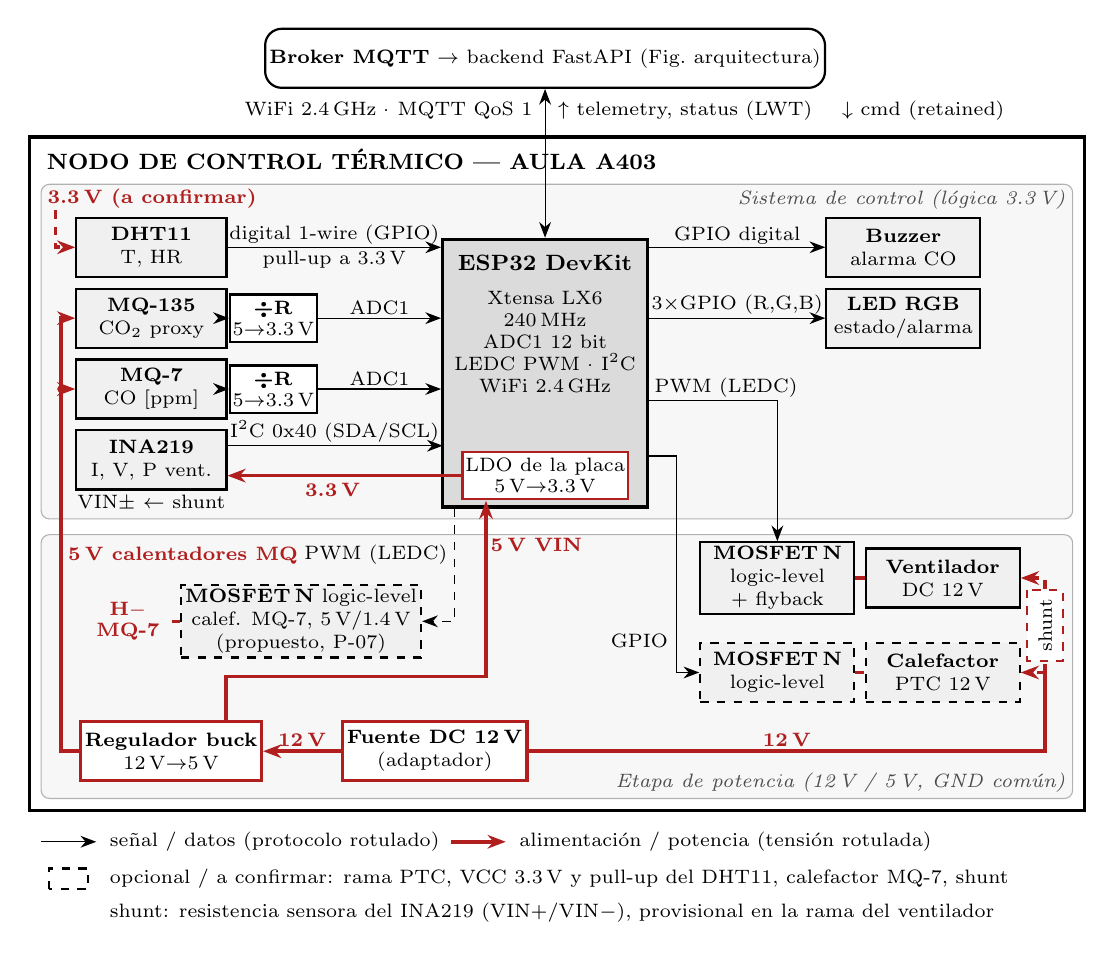
\begin{tikzpicture}

% ================= Grupos (fondo, coordenadas explicitas) =================
\begin{scope}[on background layer]
  \draw[very thick] (-6.55,-5.0) rectangle (6.85,3.55);                 % nodo
  \draw[grupo] (-6.40,-1.30) rectangle (6.70,2.95);                     % control
  \draw[grupo] (-6.40,-4.85) rectangle (6.70,-1.50);                    % potencia
\end{scope}
\node[anchor=west, font=\fontsize{8}{9}\selectfont\bfseries] at (-6.45,3.27)
  {NODO DE CONTROL TÉRMICO — AULA A403};
\node[grupolbl, anchor=north east] at (6.65,2.92) {Sistema de control (lógica 3.3\,V)};
\node[grupolbl, anchor=south east] at (6.65,-4.82) {Etapa de potencia (12\,V / 5\,V, GND común)};

% ================= MCU (centro) =================
\node[mcu] (esp) at (0,0.55) {};
\node[font=\fontsize{8.5}{9.5}\selectfont\bfseries] at (0,1.95) {ESP32 DevKit};
\node[align=center, font=\fontsize{7}{8}\selectfont] at (0,0.95)
  {Xtensa LX6\\240\,MHz\\ADC1 12 bit\\LEDC PWM · I\textsuperscript{2}C\\WiFi 2.4\,GHz};
\node[iface, draw=acento, thick, minimum width=21mm] (ldo) at (0,-0.75) {LDO de la placa\\5\,V$\rightarrow$3.3\,V};

% ================= Entradas (izquierda) =================
\node[sensor] (dht)   at (-5.0, 2.15) {\textbf{DHT11}\\T, HR};
\node[sensor] (mq135) at (-5.0, 1.25) {\textbf{MQ-135}\\CO\textsubscript{2} proxy};
\node[sensor] (mq7)   at (-5.0, 0.35) {\textbf{MQ-7}\\CO [ppm]};
\node[sensor] (ina)   at (-5.0,-0.55) {\textbf{INA219}\\I, V, P vent.};
\node[lbl, anchor=north] at ($(ina.south)+(0,-0.02)$) {VIN$\pm$ $\leftarrow$ shunt};

\node[iface] (div1) at (-3.45, 1.25) {\textbf{÷R}\\5$\rightarrow$3.3\,V};
\node[iface] (div2) at (-3.45, 0.35) {\textbf{÷R}\\5$\rightarrow$3.3\,V};

\draw[data] (dht.east)   -- node[lbl, above] {digital 1-wire (GPIO)} node[lbl, below, pos=0.5] {pull-up a 3.3\,V} (dht.east -| esp.west);
\draw[data] (mq135.east) -- (div1.west);
\draw[data] (div1.east)  -- node[lbl, above] {ADC1} (div1.east -| esp.west);
\draw[data] (mq7.east)   -- (div2.west);
\draw[data] (div2.east)  -- node[lbl, above] {ADC1} (div2.east -| esp.west);
\draw[data] (-4.05,-0.37) -- node[lbl, above] {I\textsuperscript{2}C 0x40 (SDA/SCL)} (-1.3,-0.37);
% 3.3 V del LDO hacia INA219 (lado opuesto a la flecha I2C, sin cruce)
\draw[pwr] (ldo.west) -- node[tag, below=1pt, pos=0.55] {3.3\,V} ($(ina.east)+(0,-0.2)$ |- ldo.west);

% ================= Salidas de senal (derecha, arriba) =================
\node[actuator] (buz) at (4.55, 2.15) {\textbf{Buzzer}\\alarma CO};
\node[actuator] (rgb) at (4.55, 1.25) {\textbf{LED RGB}\\estado/alarma};
\draw[data] (buz.west -| esp.east) -- node[lbl, above] {GPIO digital} (buz.west);
\draw[data] (rgb.west -| esp.east) -- node[lbl, above] {3$\times$GPIO (R,G,B)} (rgb.west);

% ================= Etapa de potencia =================
\node[actuator] (q1)  at (2.95,-2.05) {\textbf{MOSFET\,N}\\logic-level\\+ flyback};
\node[actuator] (fan) at (5.05,-2.05) {\textbf{Ventilador}\\DC 12\,V};
\node[actuator, confirmar] (q2)  at (2.95,-3.25) {\textbf{MOSFET\,N}\\logic-level};
\node[actuator, confirmar] (ptc) at (5.05,-3.25) {\textbf{Calefactor}\\PTC 12\,V};

\node[power] (buck)   at (-4.75,-4.25) {\textbf{Regulador buck}\\12\,V$\rightarrow$5\,V};
\node[power] (fuente) at (-1.40,-4.25) {\textbf{Fuente DC 12\,V}\\(adaptador)};

% Control de drivers (datos)
\draw[data] ($(esp.east)+(0,-0.35)$) -| node[lbl, pos=0.3, above] {PWM (LEDC)} (q1.north);
\draw[data] ($(esp.east)+(0,-1.05)$) -- ++(0.35,0) |- (q2.west);
\node[lbl, anchor=east] at (1.60,-2.85) {GPIO};

% Conmutacion lado bajo: driver <-> carga
\draw[pwr, -] (q1.east) -- (fan.west);
\draw[pwr, -, dashed] (q2.east) -- (ptc.west);

% Rama 12 V: fuente -> bus derecho -> cargas (shunt INA219 en rama ventilador)
\draw[pwr, -] (fuente.east) -- node[tag, above, pos=0.5] {12\,V} (6.35,-4.25) -- (6.35,-3.25);
\draw[pwr, dashed] (6.35,-3.25) -- (ptc.east);
\node[iface, draw=acento, thick, dashed, rotate=90, minimum width=9mm, minimum height=4.5mm,
      font=\fontsize{7}{7}\selectfont] (shunt) at (6.35,-2.65) {shunt};
\draw[pwr, -, dashed] (6.35,-3.25) -- (shunt.west);
\draw[pwr, dashed] (shunt.east) |- (fan.east);

% Rama 5 V: fuente -> buck -> ESP32 VIN (LDO) y calentadores MQ / DHT11
\draw[pwr] (fuente.west) -- node[tag, above] {12\,V} (buck.east);
\draw[pwr] ($(buck.north)+(0.7,0)$) |- (-0.75,-3.3) -- node[tag, right, pos=0.75] {5\,V VIN} (-0.75,-1.07);
\draw[pwr] (buck.west) -| (-6.15,1.25) -- (mq135.west);
\draw[pwr, dashed] (-6.15,0.35) -- (mq7.west);
\fill[acento] (-6.15,0.35) circle (1.3pt);
\draw[pwr, dashed] (-6.22,2.62) -- (-6.22,2.15) -- (dht.west);
\node[tag, anchor=south west] at (-6.36,2.60) {3.3\,V (a confirmar)};
\node[tag, anchor=north west, align=left] at (-6.10,-1.62) {5\,V calentadores MQ};

% DIA-3-03: calefactor MQ-7 ciclado 5 V/1.4 V por MOSFET + canal LEDC (propuesto, P-07).
% Salida como etiqueta de red (H- MQ-7) para no cruzar I2C ni 3.3 V.
\node[base, fill=gray!12, confirmar, minimum width=28mm] (q3) at (-3.1,-2.6)
  {\textbf{MOSFET\,N} logic-level\\calef. MQ-7, 5\,V/1.4\,V\\(propuesto, P-07)};
\draw[data, dashed] ($(esp.south west)+(0.17,0)$) |- (q3.east);
\node[lbl, anchor=east] at (-1.2,-1.75) {PWM (LEDC)};
\draw[pwr, -, dashed] (q3.west) -- ++(-0.2,0) node[tag, anchor=east, align=center] {H$-$\\MQ-7};

% ================= WiFi / MQTT (arriba, fuera del nodo) =================
\node[base, fill=white, rounded corners=6pt, minimum width=52mm] (broker) at (0,4.55)
  {\textbf{Broker MQTT} $\rightarrow$ backend FastAPI (Fig.~arquitectura)};
\draw[{Stealth[length=2mm]}-{Stealth[length=2mm]}, thin] (esp.north) -- (broker.south);
\node[lbl, anchor=east] at (-0.12,3.88) {WiFi 2.4\,GHz · MQTT QoS 1};
\node[lbl, anchor=west] at (0.12,3.88) {$\uparrow$ telemetry, status (LWT) \quad $\downarrow$ cmd (retained)};

% ================= Leyenda =================
\begin{scope}[shift={(-6.4,-5.4)}, font=\fontsize{7}{7.5}\selectfont]
  \draw[data] (0,0) -- (0.7,0); \node[anchor=west] at (0.75,0) {señal / datos (protocolo rotulado)};
  \draw[pwr]  (5.2,0) -- (5.9,0); \node[anchor=west] at (5.95,0) {alimentación / potencia (tensión rotulada)};
  \draw[thick, dashed] (0.1,-0.6) rectangle (0.6,-0.34);
  \node[anchor=west] at (0.75,-0.47) {opcional / a confirmar: rama PTC, VCC 3.3\,V y pull-up del DHT11, calefactor MQ-7, shunt};
  \node[anchor=west] at (0.75,-0.9) {shunt: resistencia sensora del INA219 (VIN+/VIN$-$), provisional en la rama del ventilador};
\end{scope}

\end{tikzpicture}
\end{document}
